\documentclass[a4paper,12pt]{article}
\usepackage[utf8]{inputenc}
\usepackage[brazil]{babel}
\usepackage[parfill]{parskip} % Activate to begin paragraphs with an empty line rather than an indent

\usepackage{graphicx} % support the \includegraphics command and options
\usepackage{url} % support the url references

\usepackage{fancyvrb} % better looking verbatim

\usepackage{float}

%font
\usepackage{times}
% \usepackage{mathptmx}
\usepackage[T1]{fontenc}

% to adjust figures numbering
% \usepackage{amsmath}
% \numberwithin{figure}{section}

% %figura
% \begin{figure}[h]
% \centering
% \includegraphics[width=\linewidth]{imgs/.png}
% \label{fig:}
% \caption{}
% \end{figure}


\author{Alberto Vital Santos de Sousa}

\begin{document}
%================CAPA===================
\pagenumbering{gobble} % turn off page numbering
\begin{center}
\begin{figure}[h]
\centering

\includegraphics[width=3cm]{imgs/ufpe.png}

\includegraphics[width=4cm]{imgs/cin.png}
\end{figure}
%{\Large
Universidade Federal de Pernambuco\\
Centro de Informática\\
Curso de Bacharelado em Engenharia da Computação
%}
\\[3cm]
\textbf{\huge
AndroidDriller:\\[3mm]
Uma ferramenta de mineração de repositórios Android\\
}
\vfill
\begin{flushleft}
Aluno: Alberto Vital Santos de Sousa\\
Orientador: Leopoldo Motta Teixeira\\[5mm]
\end{flushleft}
Recife, junho de 2018
\end{center}

%================ContraCapa===================
\newpage
\begin{center}
Universidade Federal de Pernambuco\\
Centro de Informática\\
Curso de Bacharelado em Engenharia da Computação
%}
\\[3cm]
\textbf{\huge
AndroidDriller:\\[3mm]
Uma ferramenta de mineração de repositórios Android\\
}
\vfill

\begin{flushleft}
{\small
Monografia apresentada ao Centro de Informática (CIn)\\
da Universidade Federal de Pernambuco (UFPE), como requisito\\
parcial para conclusão do Curso de Engenharia da Computação,\\
orientada pelo professor Leopoldo Motta Teixeira.
}
\end{flushleft}
Recife, junho de 2018
\end{center}


%================AGRADECIMENTOS===================
\newpage
\section*{Agradecimentos}

São muitos nomes para que eu me lembre de todos os que merecem aqui, mas gostaria de agradecer àqueles que de alguma forma contribuíram não só para este trabalho como também para a minha formação como pessoa. Em especial posso citar meus pais Antonio Vital Alves de Sousa e Maria Auxiliadora Santos Vital Alves de Sousa, que sempre me apoiaram e me incentivaram nas minhas decisões e a sempre seguir com meus estudos. Também agradeço ao meu orientador Leopoldo Motta Teixeira, pelos suporte e ensinamentos que me proporcionou durante este período. De uma maneira geral agradeço também a todos os meus colegas de graduação e do laboratório Oki Brasil, que estiveram ao meu lado durante os momentos difíceis da graduação e também nos de  descontração do dia a dia.

%================RESUMO===================
\newpage
\pagenumbering{arabic} % turn page numbering back on
\section*{Resumo}
Utilizando ferramentas capazes de minerar dados sobre repositórios, pesquisadores de engenharia de software têm obtido um melhor conhecimento sobre o processo de desenvolvimento de software, em geral. Este trabalho propõe uma ferramenta capaz de minerar repositórios fazendo uso das características comuns de projetos Android para que se possa realizar uma investigação preliminar de como as mudanças acontecem no desenvolvimento de aplicações para a plataforma. Por fim, são apresentados os resultados da utilização da ferramenta sobre um conjunto de mais de 1100 repositórios Android livres e de código aberto retirados do catálogo do f-droid. 

\textbf{Palavras-chave}: Android, Mineração de Repositórios, Sistema de Controle de Versão, Git

%================ABSTRACT===================
\newpage
\section*{Abstract}

Software Engineering researchers have been using tools capable of mining data from repositories to get a better understanding about the software development process. This work proposes a tool for mining repositories that uses the common characteristics of Android Projects so we can perform a preliminary investigation about how changes occur in the platform apps development. In the end, we present the results of running the tool over a set of more than 1100 free and open source Android repositories taken from the f-droid catalogue. 

\textbf{Keywords}: Android, Repository Mining, Version Control System, Git

%================Sumario===================
\newpage

\tableofcontents

%================INTRODUÇÃO===================
\newpage
\section{Introdução}

Em engenharia de software, a análise de repositórios tem ajudado pesquisadores a obter um melhor conhecimento sobre o processo de desenvolvimento de um software \cite{miningGit}, pois a análise de software consiste em extrair dados para que gerentes e engenheiros de software possam melhorar os processos de tomada de decisão e desenvolvimento de softwares \cite{soWhat}. Dessa forma, podemos definir como mineração de repositórios o processo de  extração desses dados. Com isso, é possível predizer bugs e também analisar o padrão de desenvolvimento utilizado pelos colaboradores do projeto. Para tal fim, existem ferramentas capazes de minerar dados sobre repositórios, como por exemplo, o RepoDriller \cite{repodriller}.\\
\\
Ferramentas mais gerais, como o próprio RepoDriller, servem para analisar software em vários domínios. No desenvolvimento de aplicações Android, há diversas particularidades envolvidas. Por exemplo, o arquivo de manifesto, chamado AndroidManifest, é obrigatório para qualquer aplicação da plataforma e contém informações sobre os vários componentes do projeto. Assim, qualquer componente não declarado aqui também não fará parte da aplicação final, da mesma forma que permissões utilizadas no código precisam ser declaradas neste arquivo para que funcionem corretamente. Com isso, as principais alterações feitas no repositório são refletidas em modificações desse arquivo, o que pode ser utilizado para mineração de dados relativos ao histórico de alterações do projeto.\\
\\
No estudo de repositórios Android, pesquisadores têm usado ferramentas capazes
de extrair dados dos arquivos do tipo apk \cite{Calciati}, \cite{WhoAdded} e \cite{YLyu}. Para realizar estudos
semelhantes, uma outra abordagem seria utilizar uma ferramenta capaz de
minerar os repositórios das aplicações e extrair dados específicos levando em
consideração não só o arquivo apk mas também as modificações dos arquivos de
manifesto, por exemplo.\\


%================OBJETIVOS===================

\subsection{Objetivos}

Este trabalho tem por objetivo realizar uma investigação preliminar de como as mudanças acontecem no desenvolvimento de aplicações Android para criar ferramentas de suporte à evolução de aplicativos, e assim, implementar uma ferramenta capaz de minerar estes repositórios, aproveitando-se das características particulares de projetos Android.\\


%=============================
%=      Desenvolvimento      =
%=============================

%================CONCEITOSBASICOS===================
\newpage

\section{Conceitos Básicos}

Neste capítulo apresentamos conceitos essenciais para a compreensão do trabalho. Na Seção \ref{sec:android} apresentamos a plataforma Android e seus componentes. Na Seção \ref{sec:scv} explicamos o que são sistemas de controle de versão, destacando o Git.  Na seção seguinte comentamos sobre mineração de repositórios, e por fim, ainda na Seção \ref{sec:mining}, apresentamos o framework utilizado para desenvolver a ferramenta proposta.

\subsection{Android}%10
%o que é android
\label{sec:android}
O sistema operacional Android pode ser definido como uma pilha de software de código aberto desenvolvida para sistemas móveis \cite{androidSource}. A partir desta pilha, programadores são capazes de desenvolver aplicações para dispositivos móveis sem se preocupar com detalhes específicos de hardware, pois a própria plataforma trata essas diferenças em sua API. O fato de Android ter seu código aberto, também permite ao desenvolvedor implementar sua própria versão dos módulos da plataforma caso deseje.

A pilha de software citada acima pode ser dividida em camadas, conforme a Figura \ref{fig:androidStack}

%figura dos modulos
\begin{figure}[h]
\centering
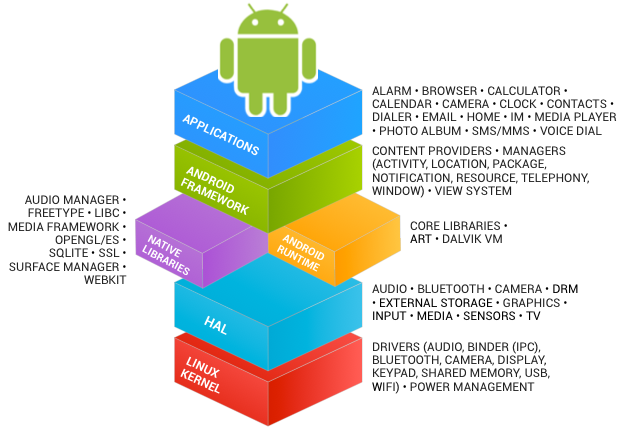
\includegraphics[width=0.8\linewidth]{imgs/android_framework_details.png}
\caption{Pilha de software dividida em camadas \cite{androidSource}}
\label{fig:androidStack}
\end{figure}


A camada mais inferior, \textit{Linux Kernel}, provê uma abstração do hardware para as camadas superiores, com os serviços mais genéricos de um sistema operacional. Na camada \textit{HAL} ou \textit{Hardware Abstraction Layer}, temos uma abstração maior do hardware, realizando o carregamento dos drivers específicos para os periféricos solicitados pelas camadas superiores. Nas camadas \textit{Native Libraries} e \textit{Android Runtime}, encontram-se as bibliotecas nativas e a máquina virtual que roda as aplicações. Na camada \textit{Android Framework}, encontram-se os principais elementos providos pela plataforma para as aplicações, como por exemplo as notificações. Na camada superior, denominada \textit{Applications} é onde estão as aplicações e as principais classes utilizadas pelos desenvolvedores para produzi-las. \\

Este trabalho propõe uma ferramenta para extrair dados relativos à camada \textit{Applications}. Mais abaixo trataremos alguns dos principais elementos da plataforma e que são abordados pela ferramenta proposta.


%detalhamento dos componentes
%olhar pagina do android developer
\subsubsection{AndroidManifest}
%O core da ferramenta
É um arquivo XML obrigatório que contém informações sobre os componentes da aplicação. Precisa ser criado com o nome {\small\texttt{\textbf{AndroidManifest.xml}}}, dessa forma a plataforma é capaz de identificar, dentre outras coisas, qual parte do código implementa a cada uma das entidades que compõem a aplicação. Assim, qualquer componente utilizado no código precisa ser declarado neste arquivo para que funcione corretamente, analogamente, qualquer componente não declarado aqui também não fará parte da aplicação final. Um exemplo desse arquivo pode ser visto na Figura \ref{fig:manifest}.

 %figura de manifesto
 \begin{figure}[h]
 \centering
 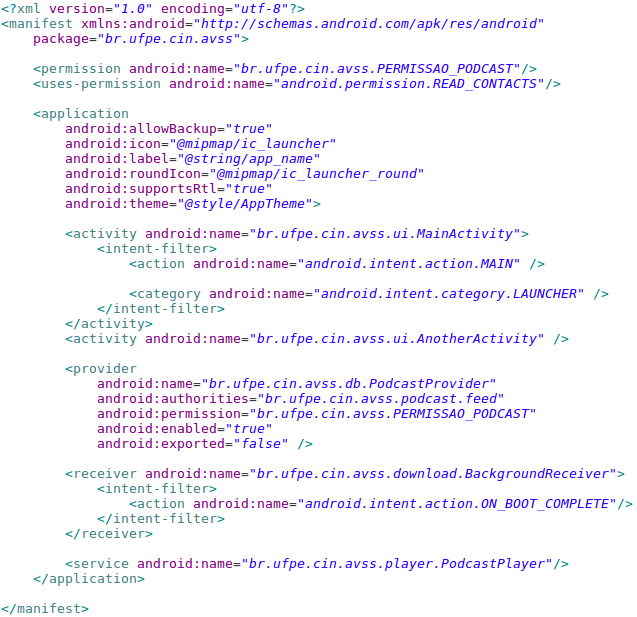
\includegraphics[width=\linewidth]{imgs/manifest.png}
 \caption{Exemplo de arquivo AndroidManifest.xml}
 \label{fig:manifest}
 \end{figure}



\subsubsection{Activity}
É o componente que representa a interface visual de interação com o usuário. No arquivo de manifesto é representada pela tag {\small\texttt{\textbf{activity}}} e precisa definir o atributo {\small\texttt{\textbf{name}}}, que é utilizado para identificar a classe que a implementa.\\

Na Figura \ref{fig:manifest} podemos ver duas activities sendo declaradas, uma delas possui o atributo {\small\texttt{\textbf{name}}} definido como {\small\texttt{\textbf{br.ufpe.cin.avss.ui.AnotherActivity}}}.
{\fontsize{9pt}{12pt}
\begin{Verbatim}
<activity android:name="br.ufpe.cin.avss.ui.AnotherActivity" />
\end{Verbatim}
}

Dessa forma, a plataforma espera encontrar no pacote {\small\texttt{\textbf{br.ufpe.cin.avss.ui}}} a implementação da classe {\small\textbf{\texttt{AnotherActivity}}} que representará uma das telas da aplicação.

\subsubsection{Broadcast Receiver}

A plataforma Android utiliza um sistema de eventos similar ao padrão \textit{publish-subscribe}, onde a plataforma (ou outra aplicação) dispara um evento (\textit{broadcast}) e as aplicações registradas para o evento recebem a mensagem correspondente. O componente que recebe estes eventos é conhecido como \textit{broadcast receiver}.\\
\\
Ao iniciar o dispositivo, o sistema android dispara um evento de \textit{broadcast} chamado de {\small\texttt{\textbf{ON\_BOOT\_COMPLETE}}}. Para que a aplicação receba esse e outros eventos semelhantes é necessário implementar uma classe do tipo {\small\texttt{\textbf{BroadcastReceiver}}} e registrá-la no evento desejado. Para isso, declara-se no manifesto a tag {\small\texttt{\textbf{receiver}}}, conforme o trecho abaixo, que também pode ser visto na Figura \ref{fig:manifest} onde foi declarado um componente receiver que espera eventos do tipo citado anteriormente.
{\fontsize{9pt}{12pt}
\begin{verbatim}
<receiver android:name="br.ufpe.cin.avss.download.BackgroundReceiver">
  <intent-filter>
    <action android:name="android.intent.action.ON_BOOT_COMPLETE"/>
  </intent-filter>
</receiver>
\end{verbatim}
}

\subsubsection{Content Provider}
\label{sec:provider}
Componente responsável por prover uma interface de acesso para outras aplicações aos dados utilizados. Dessa forma, cria-se uma abstração da camada de dados que pode ser utilizada não só por outras aplicações como também pela própria aplicação, conectando os dados em um processo com o código em execução em outro.\\

No manifesto é representada pela tag {\small\texttt{\textbf{provider}}}. Na Figura \ref{fig:manifest} temos um exemplo que foi replicado no trecho abaixo, onde a exemplo da tag {\small\texttt{\textbf{activity}}}, o atributo {\small\texttt{\textbf{name}}} define a classe com a implementação correspondente.\\

{\fontsize{9pt}{12pt}
\begin{verbatim}
<provider
    android:name="br.ufpe.cin.avss.db.PodcastProvider"
    android:authorities="br.ufpe.cin.avss.podcast.feed"
    android:permission="br.ufpe.cin.avss.PERMISSAO_PODCAST"
    android:enabled="true"
    android:exported="true" />

\end{verbatim}
}


Ao declarar este elemento é necessário definir o atributo {\small\texttt{\textbf{authorities}}}, que seguindo a convenção de nomes em Java, identifica o provider declarado. Em geral, esse nome é baseado no package name da aplicação, que deve ser único dentre todas as aplicações da plataforma. Dessa forma, os providers declarados pelas aplicações podem ser exportados, pois, a plataforma irá identificá-los a partir do atributo {\small\texttt{\textbf{authorities}}}.\\

O atributo {\small\texttt{\textbf{permission}}} define que para acessar os dados deste receiver, é necessário possuir a permissão {\small\texttt{\textbf{br.ufpe.cin.avss.PERMISSAO\_PODCAST}}}, um elemento que será discutido mais à frente.




\subsubsection{Service}



Este componente não provê uma interface visual e roda em background. Dessa forma, é utilizado para implementar procedimentos  que não necessitam que a aplicação esteja ativa no momento. Em geral, operações mais pesadas como downloads de arquivos e reprodução de áudio são realizadas por estes componentes, uma vez que sua execução não é finalizada mesmo quando o usuário sai da aplicação. No manifesto é declarado com a tag {\small\texttt{\textbf{service}}}, como pode ser visto no trecho abaixo retirado da Figura \ref{fig:manifest}.
{\fontsize{9pt}{12pt}
\begin{verbatim}
<service android:name="br.ufpe.cin.avss.player.PodcastPlayer"/>
\end{verbatim}
}

\subsubsection{Permission}
%tratar uses-permission aqui
O sistema de permissões da plataforma Android garante que certas ações só sejam executadas caso o usuário da aplicação conceda o privilégio necessário. As permissões podem ser classificadas em:
\begin{itemize}
    \item {Dangerous}
    \item {Normal}
    \item {Signature}
    \item {Signature or System}
\end{itemize}


As permissões consideradas \textit{dangerous} podem causar algum risco à privacidade do usuário ou ao funcionamento normal do dispositivo, por isso necessitam da validação do usuário. As \textit{normal}, por não trazerem esses riscos, são concedidas automaticamente pelo sistema ao serem declaradas no manifesto.\\

Desde a versão 6.0 da plataforma Android, a forma como as permissões são solicitadas foi alterada. Nas versões anteriores, qualquer permissão \textit{dangerous} é solicitada antes da instalação, e caso a aplicação precise ser atualizada, as permissões são solicitadas novamente. Caso o usuário não conceda alguma permissão, a aplicação não é instalada nem atualizada. A partir da versão 6.0, as permissões \textit{dangerous} são solicitadas em tempo de execução. Dessa forma, a aplicação pode ser instalada sem que o usuário tenha que conceder todos os privilégios solicitados. Assim,  a permissão associada com a funcionalidade ativada é solicitada sempre que o usuário desejar utilizar a funcionalidade.\\

Dessa forma, caso uma aplicação deseje ler os contatos do usuário, por exemplo, é necessário declarar a tag {\small\texttt{\textbf{uses-permission}}} no manifesto com o atributo {\small\texttt{\textbf{name}}} de valor igual a {\small\texttt{\textbf{"android.permission.READ\_CONTACTS"}}}, conforme pode ser visto na Figura \ref{fig:manifest}.

{\fontsize{9pt}{12pt}
\begin{verbatim}
<uses-permission android:name="android.permission.READ_CONTACTS"/>
\end{verbatim}
}


%tratar das permissoes criadas pela aplicação
Existe também a possibilidade da própria aplicação definir permissões de acesso ao seus conteúdos. Para isso, utiliza-se a tag {\small\texttt{\textbf{permission}}}. Conforme foi visto na Seção \ref{sec:provider}, o atributo {\small\texttt{\textbf{permission}}} pode ser utilizado para definir uma permissão de acesso ao conteúdo provido pelo componente. Dessa forma, pode-se notar que a aplicação definida no arquivo da Figura \ref{fig:manifest} não só define uma permissão própria, como também protege seu content provider com essa mesma permissão, de acordo com as tags do trecho abaixo.

{\fontsize{9pt}{12pt}
\begin{verbatim}
<permission android:name="br.ufpe.cin.avss.PERMISSAO_PODCAST"/>
...
<provider
    android:name="br.ufpe.cin.avss.db.PodcastProvider"
    android:authorities="br.ufpe.cin.avss.podcast.feed"
    android:permission="br.ufpe.cin.avss.PERMISSAO_PODCAST"
    android:enabled="true"
    android:exported="false" />
\end{verbatim}
}



%\newpage
\subsection{Sistemas de controle de versão}%11-15
\label{sec:scv}
São sistemas que controlam o versionamento de um software durante o estágio de desenvolvimento. Com estes sistemas é possível saber qual o estado exato do código fonte em um determinado período do processo de produção, pois a cada alteração realizada o sistema armazena quais arquivos e quais linhas foram modificadas naquele momento, além de também informar quem realizou as alterações.\\

Na próxima seção apresentamos o Git, um dos mais populares sistemas de controle de versão da atualidade.

\subsubsection{Git}%11-17
%\newpage
É um sistema de controle de versão descentralizado livre e de código aberto \cite{git}, onde cada desenvolvedor tem uma cópia completa do histórico do repositório. A cada conjunto de  alterações registrada  um \textit{snapshot} do projeto denominado \textit{commit} é armazenado. O git utiliza uma estrutura de grafos para organizar os commits em diversas linhas de desenvolvimento, cada uma sendo denominada \textit{branch} \cite{gitHandbook}.

Abaixo estão listados alguns dos principais comandos git, juntamente com uma breve explicação de seu funcionamento.

\begin{itemize}
\item{{\small\texttt{git init}} } Inicializa um repositório a partir de um diretório local.
\item{{\small\texttt{git clone}} } Copia um repositório remoto em um diretório local.
\item{{\small\texttt{git pull}} } Recupera as mudanças remotas para o repositório local.
\item{{\small\texttt{git add}} } Adiciona as mudanças locais num conjunto para que possam ser incluídas no próximo commit.
\item{{\small\texttt{git commit}} } Cria um commit com as mudanças selecionadas pelo comando git add.
\item{{\small\texttt{git push}} } Atualiza o repositório remoto remoto com as mudanças locais.
\item{{\small\texttt{git branch}} } Cria uma nova linha de desenvolvimento
\item{{\small\texttt{git merge}} } Unifica duas linhas de desenvolvimento em um novo commit que é denominado \textit{merge commit}
\end{itemize}

Para exemplificar o funcionamento de um merge commit, suponha o seguinte grafo de commits de um repositório representado pela Figura \ref{fig:graphBefore}.

 %figura
 \begin{figure}[h]
 \centering
 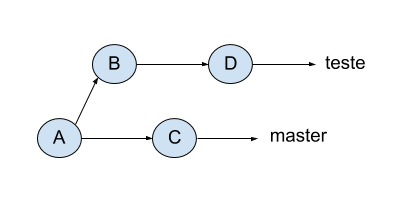
\includegraphics[width=0.65\linewidth]{imgs/graph_before.png}
 \caption{Grafo de commits com duas branches}
 \label{fig:graphBefore}
 \end{figure}



Estando na branch master e executando o comando {\small\texttt{\textbf{git merge teste}}} cria-se o commit \textit{E} na branch master e que unifica as modificações realizadas nas duas branches, resultando no grafo da Figura \ref{fig:graphAfter}.

 %figura
 \begin{figure}[H]
 \centering
 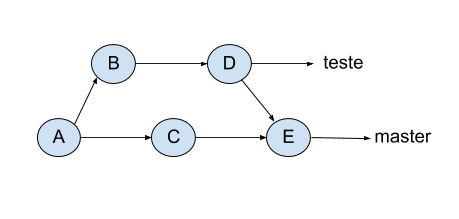
\includegraphics[width=0.65\linewidth]{imgs/graph_after.png}
 \caption{Grafo de commits após o merge commit 'E'.}
 \label{fig:graphAfter}
 \end{figure}


\subsection{Mineração de repositórios}%11-15
\label{sec:mining}



A análise de software consiste em extrair dados para que gerentes e engenheiros de software possam melhorar o processo de desenvolvimento de software através do ganho e compartilhamento de ideias provenientes desses dados para uma melhor tomada de decisão \cite{soWhat}. Dessa forma, podemos definir como mineração de repositórios o processo de  extração desses dados. Devido ao tamanho e a quantidade de repositórios utilizados durante seus estudos, pesquisadores têm utilizado ferramentas de mineração para automatizar esse processo. %\cite{something I don't know yet}.
\\
\\
Na próxima seção apresentamos uma ferramenta utilizada para minerar repositórios, e que foi utilizada como base para a ferramenta desenvolvida neste trabalho.

%%%%%%%%%
%citar crescente dos dados -> uso de ferramentas de mineração.

%\newpage
\subsubsection{RepoDriller}%14-16
\label{sec:repodriller}
RepoDriller é um framework de mineração de repositórios feito em Java  \cite{repodriller}. Com esta ferramenta é possível extrair dados não só dos commits realizados (como por exemplo autor e mensagem) mas também dos arquivos contidos no repositório.

Para escrever um programa que minere um dado repositório, é preciso implementar a interface {\small\texttt{\textbf{Study}}} e no método {\small\texttt{\textbf{execute}}} criar um objeto de estudo (uma instância da classe {\small\texttt{\textbf{RepositoryMining}}}) utilizando o padrão builder e informando além do repositório a ser minerado, as implementações da interface {\small\texttt{\textbf{CommitVisitor}}}.  Para informar o repositório, utilizamos o método {\small\texttt{\textbf{in}}} que recebe uma implementação de  {\small\texttt{\textbf{SCMRepository}}}, podendo ser tanto Git quanto SVN. Neste trabalho foi utilizado a implementação {\small\texttt{\textbf{GitRemoteRepository}}} que recebe uma URL referenciando o repositório remoto, ver Figura \ref{fig:repostudy}.

A interface {\small\texttt{\textbf{CommitVisitor}}} define o método {\small\texttt{\textbf{process}}} que é chamado pela API interna do RepoDriller a cada commit visitado. O método {\small\texttt{\textbf{process}}} recebe como parâmetros {\small\texttt{\textbf{SCMRepository}}}, {\small\texttt{\textbf{Commit}}} e {\small\texttt{\textbf{PersistenceMechanism}}}. O primeiro é um objeto representando o repositório estudado, podendo ser Git ou SVN. O segundo é uma representação do commit sendo visitado. E o terceiro é um objeto para tratar a persistência dos dados minerados ao longo dos vários commits visitados.

Ainda no objeto {\small\texttt{\textbf{RepositoryMining}}}, definimos o mecanismo de persistência a ser passado para cada visitor. Em geral, escolhe-se um arquivo CSV. A partir da versão 1.4 do RepoDriller, pode-se definir uma configuração de coleta, para evitar que dados desnecessários sejam carregados a cada commit. Para o nosso caso em que vamos focar em informações básicas do commit e nas modificações do arquivo de manifesto, foi acrescentada a chamada ao método  {\small\texttt{\textbf{collect}}} como pode ser visto na Figura \ref{fig:repostudy}.


%figura do objeto RepositoryMining.
\begin{figure}[h]
\centering
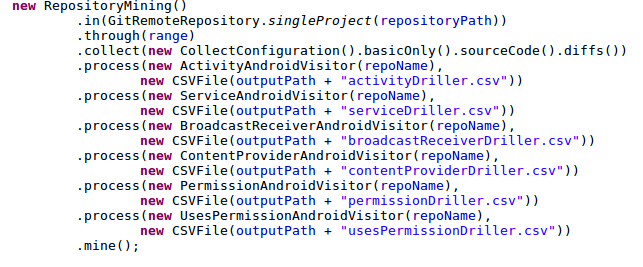
\includegraphics[width=\linewidth]{imgs/repostudy.png}
\caption{Objeto {\small\texttt{\textbf{RepositoryMining}}} definido no método {\small\texttt{\textbf{execute}}} da classe {\small\texttt{\textbf{RepoStudy}}}.}
\label{fig:repostudy}
\end{figure}



%================FERRAMENTA===================
\newpage
\section{AndroidDriller}%18-24
%Detalhamento geral da ferramenta

Neste capítulo apresentamos a ferramenta desenvolvida ao longo deste trabalho. Na Seção \ref{sec:metodologia} descrevemos o processo geral do que foi desenvolvido. Na Seção \ref{sec:implementacao} detalhamos cada classe implementada. Em seguida, na Seção \ref{sec:repoteste} comentamos sobre os repositórios escolhidos para validar e testar a implementação. Por fim, nas seções \ref{sec:experimentos} e \ref{sec:resultados} explicamos um experimento onde foram extraídos dados de repositórios Android com o AndroidDriller  e os resultados obtidos, respectivamente.

\subsection{Metodologia}
\label{sec:metodologia}
Foi criada uma ferramenta Java que faz uso da API provida pelo RepoDriller para percorrer os commits do repositório. Neste projeto foram implementadas as classes capazes de colher dados sobre os componentes específicos de Android e geração de relatórios em arquivos CSV. Para visualização dos dados, foi implementado um programa na linguagem Python capaz de produzir gráficos a partir dos arquivos CSV gerados pela ferramenta. Este fluxo pode ser descrito pela Figura \ref{fig:workflow}. 

 %figura
 \begin{figure}[h]
 \centering
 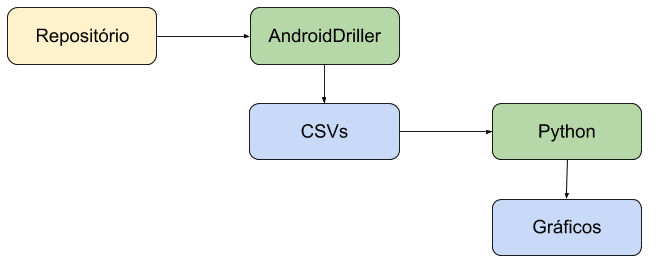
\includegraphics[width=0.65\linewidth]{imgs/workflow.png}
 \caption{Fluxo dos dados de um repositório até os gráficos gerados.}
 \label{fig:workflow}
 \end{figure}



\subsection{Implementação}%18-24
\label{sec:implementacao}


Primeiramente, vamos apresentar o modelo utilizado para representar as entidades da plataforma Android, que foi fortemente baseado no modelo utilizado em \cite{jptt}. Como pode ser visto na Figura \ref{fig:model}, temos uma classe que representa o arquivo de manifesto e cada elemento do XML foi mapeado em uma classe Java. Para representar os componentes foi utilizado o padrão de herança entre classes. Dessa forma, a classe {\small\texttt{\textbf{Component}}} contém os atributos comuns aos componentes Android, que foram representados cada um como uma classe filha de {\small\texttt{\textbf{Component}}}.\\

%figura do diagrama do modelo
\begin{figure}[H]
\centering
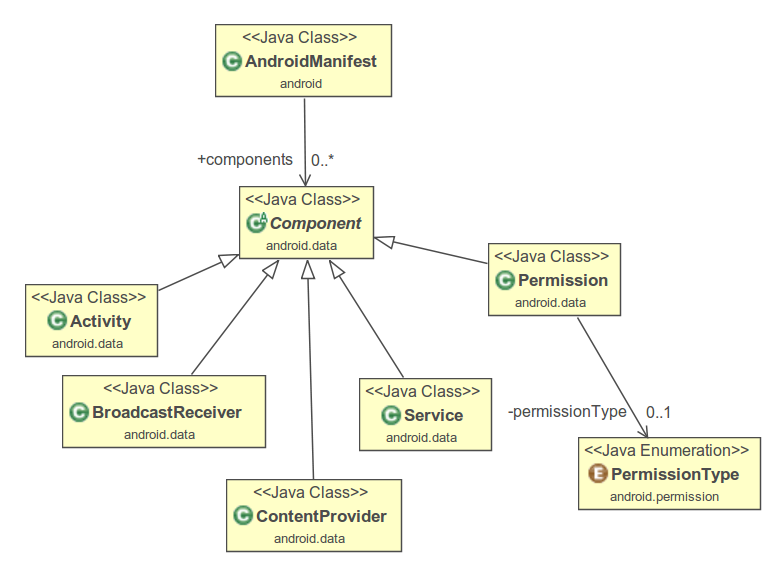
\includegraphics[width=0.8\linewidth]{imgs/model.png}
\caption{Diagrama das classes de modelo da plataforma Android.}
\label{fig:model}
\end{figure}



A classe {\small\texttt{\textbf{Component}}} também define o método {\small\texttt{\textbf{isModificationOf}}} que recebe outro componente e verifica se um é apenas uma modificação do outro ou se são componentes totalmente distintos. Para fazer essa verificação foi utilizado o atributo {\small\texttt{\textbf{name}}} como identificador do componente, ou seja, se dois componentes têm o mesmo valor de name mas valores diferentes para outros atributos, eles representam o mesmo componente apenas modificado. Por exemplo, suponha que o componente A tenha o valor de {\small\texttt{\textbf{name}}} definido como {\small\texttt{\textbf{"NomeA"}}} e o atributo {\small\texttt{\textbf{enabled}}} como {\small\texttt{\textbf{true}}}, o componente B tem {\small\texttt{\textbf{name}}} igual a {\small\texttt{\textbf{"NomeB"}}} e {\small\texttt{\textbf{enabled}}} igual a {\small\texttt{\textbf{true}}}, enquanto o componente C tem {\small\texttt{\textbf{name}}} igual a {\small\texttt{\textbf{"NomeA"}}} e {\small\texttt{\textbf{enabled}}} igual a {\small\texttt{\textbf{false}}}. Com isso, a chamada {\small\texttt{\textbf{A.isModificationOf(B)}}} retorna falso enquanto a chamada {\small\texttt{\textbf{A.isModificationOf(C)}}} retorna verdadeiro. Note que, caso exista um elemento D com {\small\texttt{\textbf{name}}} igual a {\small\texttt{\textbf{"NomeB"}}} e {\small\texttt{\textbf{enabled}}} igual a {\small\texttt{\textbf{true}}}, a chamada {\small\texttt{\textbf{D.isModificationOf(B)}}} retorna falso. Dessa forma, cada uma das subclasses de {\small\texttt{\textbf{Component}}} pode sobrescrever este método e acrescentar seus atributos específicos. Este método será útil mais à frente quando comentarmos sobre a classe {\small\texttt{\textbf{ComponentDiff}}}.

Por conveniência, os atributos e métodos foram omitidos dos diagramas aqui apresentados. %No apêndice encontram-se mais detalhes da estruturas das classes.


Seguindo uma arquitetura semelhante à das classes de modelo, foram implementadas classes de diff, conforme a Figura \ref{fig:diff}. Essas classes tratam o diff específico de cada componente. \\


%figura do diagrama dos diffs
\begin{figure}[h]
\centering
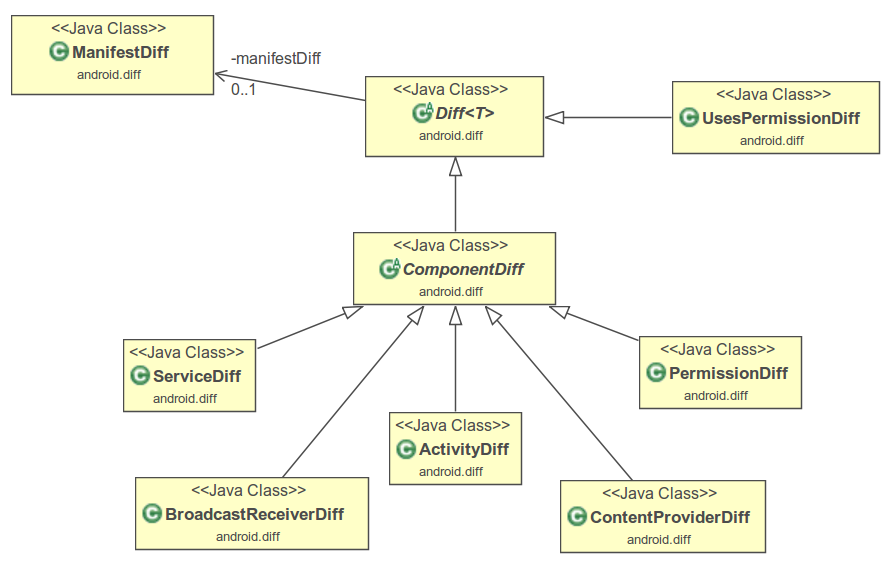
\includegraphics[width=0.8\linewidth]{imgs/diff.png}
\caption{Diagrama das classes que tratam as alterações de cada commit.}
\label{fig:diff}
\end{figure}


A classe {\small\texttt{\textbf{ManifestDiff}}} recebe uma lista de modificações registradas em cada commit, dessa lista, são filtradas as que se referem a qualquer arquivo com a denominação {\small\texttt{\textbf{AndroidManifest.xml}}}. A partir das alterações  nos manifestos, são criadas duas listas de versões dos arquivos, uma lista de arquivos anteriores e outra posteriores ao commit. De posse dessas versões utilizamos a classe {\small\texttt{\textbf{AndroidManifestParser}}} para criar duas listas de instâncias da classe {\small\texttt{\textbf{AndroidManifest}}} definida pelo modelo. As instâncias de {\small\texttt{\textbf{AndroidManifest}}} são então passadas para a classe abstrata parametrizada {\small\texttt{\textbf{Diff<T>}}} . \\


De uma forma geral, em {\small\texttt{\textbf{Diff}}} são criadas duas listas de componentes, uma representando os componentes anteriores ao commit e outra os posteriores. A partir disso, mais três listas são criadas, uma com as adições, outra com as remoções e a terceira com os componentes modificados. Para reusar o código definido nesta classe, o parâmetro {\small\texttt{\textbf{T}}} define qual componente será analisado pela subclasse de {\small\texttt{\textbf{Diff}}}, pois esta define o método abstrato {\small\texttt{\textbf{getElementsList}}} que recebe uma instância de {\small\texttt{\textbf{AndroidManifest}}} e retorna uma lista de objetos do tipo {\small\texttt{\textbf{T}}}. A classe também define outro método abstrato, {\small\texttt{\textbf{isModification}}}, que recebe um elemento {\small\texttt{\textbf{T}}} e verifica se ele foi modificado. Dessa forma, as subclasses só precisam implementar estes dois métodos para que se possa obter informações específicas de cada componente desejado. Por exemplo, a classe {\small\texttt{\textbf{UsesPermissionDiff}}} estende {\small\texttt{\textbf{Diff}}} conforme pode ser visto na Figura \ref{fig:usesdiff}, onde o parâmetro {\small\texttt{\textbf{T}}} foi definido como {\small\texttt{\textbf{String}}}, o método {\small\texttt{\textbf{getElementsList}}} apenas retorna as permissões utilizadas no manifesto e uma vez que o elemento uses-permission só define um atributo do tipo {\small\texttt{\textbf{String}}}, o método {\small\texttt{\textbf{isModification}}} retorna sempre {\small\texttt{\textbf{false}}}.
\\ 


%figura do diagrama dos diffs
\begin{figure}[h]
\centering
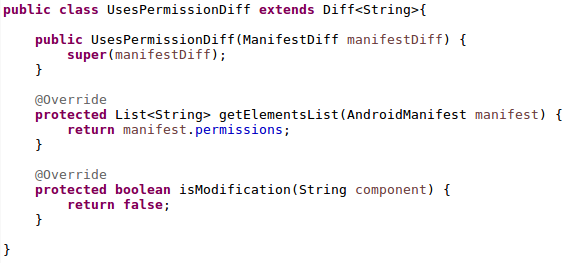
\includegraphics[width=0.8\linewidth]{imgs/usesdiff.png}
\caption{Implementação da classe {\small\texttt{\textbf{UsesPermissionDiff}}}.}
\label{fig:usesdiff}
\end{figure}




Note que na Figura \ref{fig:diff} a classe {\small\texttt{\textbf{UsesPermissionDiff}} herda diretamente da classe {\small\texttt{\textbf{Diff}}}, enquanto que os outros componentes herdam da classe {\small\texttt{\textbf{ComponentDiff}}}. Isto ocorre porque o elemento uses-permission no nosso modelo só define um atributo do tipo {\small\texttt{\textbf{String}}}, o atributo {\small\texttt{\textbf{name}}}. Por isso, ele é representado apenas como uma {\small\texttt{\textbf{String}}} com o valor desse atributo. Por esta mesma razão este componente não está representado no diagrama de modelo da Figura \ref{fig:model}. Enquanto isso, a classe abstrata {\small\texttt{\textbf{ComponentDiff}}} define o parâmetro {\small\texttt{\textbf{T}}} para ser o tipo {\small\texttt{\textbf{Component}}}, implementando o método {\small\texttt{\textbf{getElementsList}}} para retornar uma lista de {\small\texttt{\textbf{Component}}} que é recuperada pelo método abstrato {\small\texttt{\textbf{getComponents}}}, e também implementa o método {\small\texttt{\textbf{isModification}}} para retornar o {\small\texttt{\textbf{isModificationOf}}}  definido pela instância de {\small\texttt{\textbf{Component}}}, conforme vimos anteriormente. Assim as subclasses podem implementar apenas o método {\small\texttt{\textbf{getComponents}}} de forma mais específica.

%diagrama de classes
Como visto anteriormente, para percorrer os commits de um dado repositório, é preciso implementar uma interface provida pelo RepoDriller. Para que se pudesse utilizar a mesma implementação para os vários repositórios a serem minerados, foi criada a classe {\small\texttt{\textbf{RepoStudy}}}, que implementa a interface {\small\texttt{\textbf{Study}}}, conforme Figura \ref{fig:study}.

%diagrama do objeto repostudy.
\begin{figure}[h]
\centering
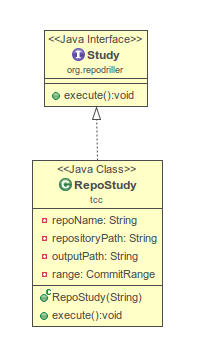
\includegraphics[width=0.3\linewidth, height=0.45\linewidth]{imgs/study.png}
\caption{Diagrama de classe do objeto RepoStudy.}
\label{fig:study}
\end{figure}

Essa classe recebe a URL do repositório a ser estudado e a partir disso inicializa o objeto {\small\texttt{\textbf{RepositoryMining}}} com o repositório a ser minerado e registra os visitors específicos de repositórios Android que serão mais detalhados à frente.


A exemplo do que foi visto na Seção \ref{sec:repodriller}, para que possamos analisar cada commit, foram implementados visitors que extraem dados a respeito de cada componente separadamente. Esses visitors seguem a estrutura definida na Figura \ref{fig:visitors}, onde um visitor abstrato implementa a interface {\small\texttt{\textbf{CommitVisitor}}} definida pelo RepoDriller, repassando a chamada do método {\small\texttt{\textbf{process}}} (que recebe um {\small\texttt{\textbf{Commit}}}) da interface para o método abstrato {\small\texttt{\textbf{androidProcess}}} (que recebe um {\small\texttt{\textbf{AndroidCommit}}}) conforme Figura \ref{fig:diagram}. Dessa forma, o {\small\texttt{\textbf{Commit}}} provido pelo framework é convertido em uma instância de {\small\texttt{\textbf{AndroidCommit}}}. Assim, a classe {\small\texttt{\textbf{DiffAndroidVisitor}}} implementa o {\small\texttt{\textbf{método androidProcess}}} e define o método abstrato {\small\texttt{\textbf{getDiff}}}, repassando o {\small\texttt{\textbf{AndroidCommit}}} para as subclasses retornarem cada uma a instância da subclasse de {\small\texttt{\textbf{Diff}}} do componente correspondente. Ainda no método {\small\texttt{\textbf{androidProcess}}}, são registrados os dados recuperados pela subclasse de {\small\texttt{\textbf{Diff}}}, retornada pelo método {\small\texttt{\textbf{getDiff}}}, no arquivo CSV definido pelo visitor utilizando a instância de {\small\texttt{\textbf{PersistenceMechanism}}} passada. Essa escrita no CSV só ocorre nos commits em que são identificadas mudanças nos arquivos de manifesto, com isso, caso um repositório possua 100 commits mas apenas 10  alteraram os manifestos, os arquivos CSV gerados terão 10 linhas cada.

A classe {\small\texttt{\textbf{AndroidCommit}}} estende a classe {\small\texttt{\textbf{Commit}}} do RepoDriller, adicionando informações específicas Android, ver Figura \ref{fig:diagram}. No seu construtor, esta classe recebe o {\small\texttt{\textbf{Commit}}} a ser estendido e o repositório a qual ele pertence, parâmetros que são utilizados para recuperar os manifestos do commit e a lista de modificações. A partir disso, é possível criar uma instância de {\small\texttt{\textbf{ManifestDiff}}}, que é utilizada como base para criação das instâncias das subclasses de {\small\texttt{\textbf{Diff}}} que serão recuperadas pelos visitors específicos, como visto anteriormente.


%figura dos visitors
\begin{figure}[h]
\centering
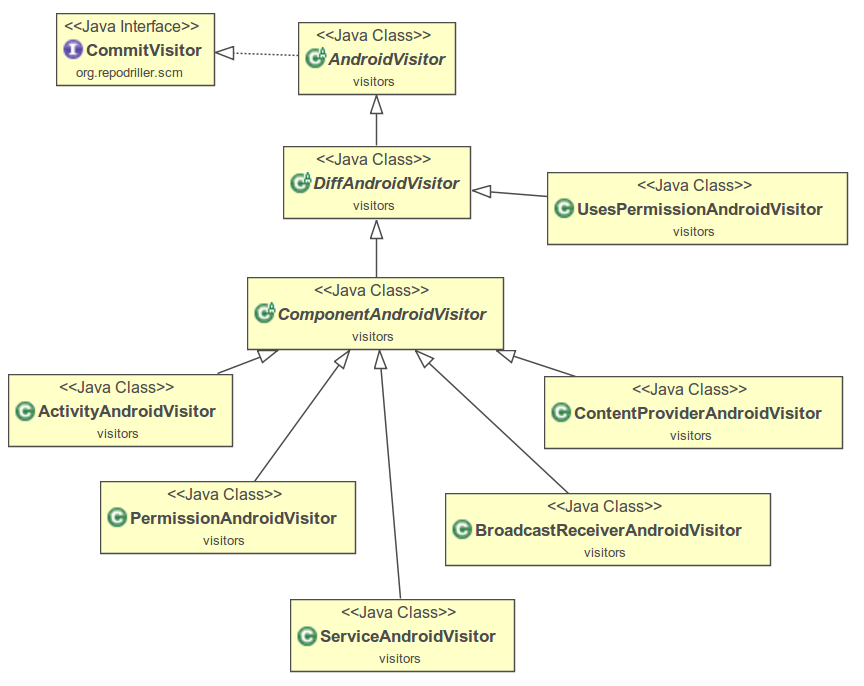
\includegraphics[width=0.8\linewidth]{imgs/visitors.png}
\caption{Diagrama das classes que implementam os visitors de cada componente.}
\label{fig:visitors}
\end{figure}


%figura do diagrama .
\begin{figure}[h]
\centering
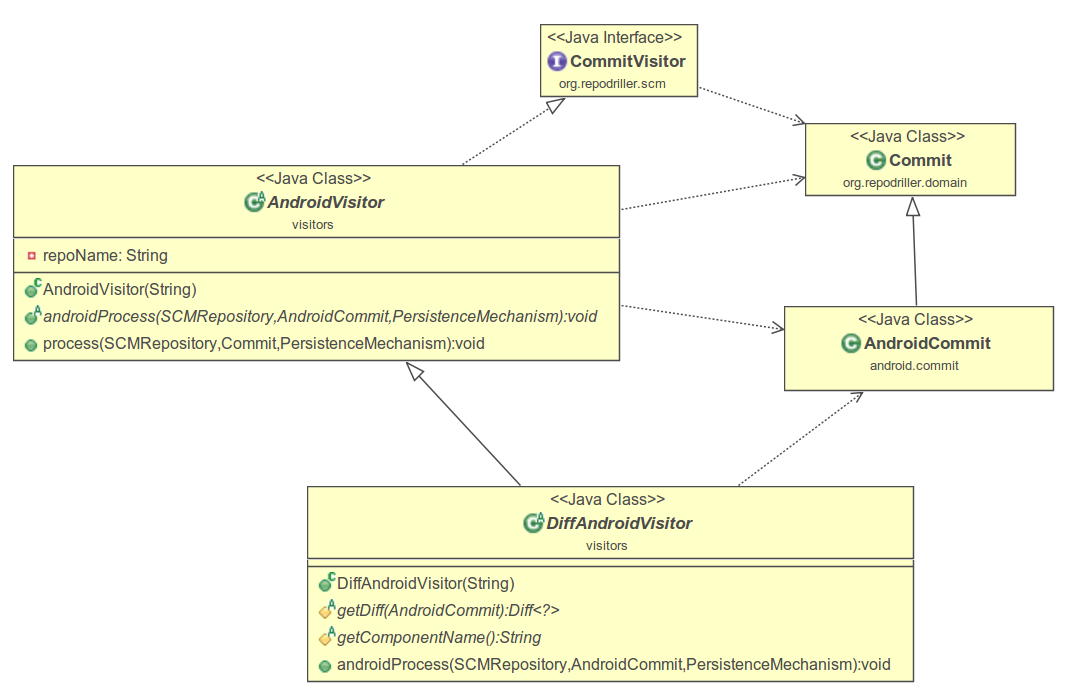
\includegraphics[width=\linewidth]{imgs/diagram.png}
\caption{Diagrama do encapsulamento do método process e da classe Commit.}
\label{fig:diagram}
\end{figure}


Para que tudo isto funcione, foi implementada a classe {\small\texttt{\textbf{MyStudy}}}, que no seu método main,  lê o arquivo de entrada encontrado na pasta {\small\texttt{\textbf{androidDriller/input}}} com o nome {\small\texttt{\textbf{repoURLs.in}}}. Este arquivo deve conter uma lista de URLs de repositórios Android remotos do github. Para cada repositório, a classe {\small\texttt{\textbf{MyStudy}}} cria uma instância de {\small\texttt{\textbf{RepoStudy}}} passando a URL do repositório como parâmetro. Na classe {\small\texttt{\textbf{RepoStudy}}}, é criado o diretório de saída, {\small\texttt{\textbf{androidDriller/output}}}, no qual são criadas uma pasta para cada repositório minerado,  onde se encontram os arquivos CSV gerados. 


%================repositórios de teste===================
\subsection{Repositórios de Teste}%18-22
\label{sec:repoteste}

No intuito de gerar um cenário pequeno, com poucos commits, mas que abrangesse os casos mais genéricos de commits que alterassem o manifesto de um aplicação, foi criado um repositório público no github apenas com 2 arquivos {\small\texttt{\textbf{AndroidManifest.xml}}} em diretórios diferentes. Neste repositório foram realizadas alterações nos dois arquivos e em branchs separadas que foram posteriormente agregadas à master e deletadas. Este repositório se encontra na URL {\fontsize{10pt}{12pt}\url{https://github.com/betosousa/fooAndroidManifest.git}}.

Para validar a implementação descrita anteriormente, foram escolhidos 6 repositórios de código livre presentes no F-Droid \cite{fdroid}, um catálogo de aplicações livre e de código aberto para a plataforma android. Juntamente com o repositório citado acima, foram listados 7 repositórios para formar uma base de testes. Esses repositórios foram escolhidos aleatoriamente dentro do catálogo, levando em conta apenas a quantidade de commits, onde tentamos escolher repositórios em faixas variadas de quantidade de commits totais.

%%%Tabela com informações dos repositórios:

\begin{table}[h]
\begin{center}
\begin{tabular}{l|c|c}

 URL & Total & Manifesto\\
\hline
https://github.com/dozingcat/AsciiCam & 56 & 28 \\
https://github.com/uberspot/2048-android & 70 & 21 \\
https://github.com/naman14/Timber & 597 & 43 \\
https://github.com/Telegram-FOSS-Team/Telegram-FOSS & 704 & 65 \\
https://github.com/jackpal/Android-Terminal-Emulator.git & 1088 & 139 \\
https://github.com/tejado/Authorizer.git & 1304 & 112 \\
https://github.com/betosousa/fooAndroidManifest.git & 29 & 24
\end{tabular}
\caption{Repositórios utilizados para validação, com quantidade total de commits e commits com alteração do manifesto.}
\end{center}
\end{table}

%%%fim Tabela%%%

Dessa forma foi possível avaliar os resultados obtidos diretamente com o histórico dos repositórios. Assim, foi possível identificar que em repositórios com commits de merge, as modificações replicadas em mais de uma branch eram contadas de forma duplicada pela ferramenta. Com isso, ao tentar calcular o total de componentes no repositório com a simples diferença entre total somado ao longo do repositório com o total removido, observamos valores diferentes do total de componentes presentes no repositório.  Para resolver isso, foi acrescentado o total de componentes por commit, que é calculado na classe {\small\texttt{\textbf{Diff}}} e representa o total de componentes na lista de elementos posteriores ao commit.


%================experimento===================
\subsection{Experimento}%18-22
\label{sec:experimentos}
%Detalhamento do experimento realizado na máquina do Cin

Para testar mais a fundo a aplicação implementada e também gerar dados para uma análise  mais profunda, foram analisados 1195 repositórios presentes no F-Droid \cite{fdroid}, cujos endereços do código fonte apontavam para o github.

Alguns repositórios apresentaram falhas durante o experimento. Foram 51 por não estarem acessíveis (ou por exigirem credenciais para clonar ou por não mais existirem) e 6 por terem arquivos de diff muito grandes, que ainda provocaram um estouro de memória e a interrupção da execução da ferramenta. Todos os 57 foram desconsiderados da análise final. 


\subsection{Resultados}%22-24
\label{sec:resultados}
Por fim, foram gerados 6 arquivos CSV para cada um dos 1138 repositórios minerados com sucesso, totalizando 49116 commits registrados com alterações no arquivo de manifesto. Na Tabela \ref{tab:statistcs} vemos um resumo dos dados coletados pela ferramenta, com a quantidade de commits que alteraram o componente, a quantidade de componentes adicionados, removidos e modificados, além do total registrado no último manifesto do repositório. Esses dados foram coletados utilizando um script Python que percorreu cada um dos arquivos CSV gerados.

\begin{table}[h]
\begin{center}
\begin{tabular}{l|c|c|c|c|c}

 Componente & Commits & Adições & Remoções & Modificações & Total \\
\hline
Activity & 16803 & 20024 & 9591 & 18419 & 6711 \\
Broadcast Receiver & 2970 & 3252 & 1542 & 1025 & 1112 \\
Content Provider & 973 & 868 & 293 & 197 & 349 \\
Service & 3019 & 3155 & 1491 & 724 & 1095 \\
Permission & 287 & 386 & 169 & 9 & 98 \\
Uses Permission & 4287 & 7253 & 1289 & 0 & 4105 \\
\end{tabular}
\caption{Resumo dos dados coletados.}
\label{tab:statistcs}
\end{center}
\end{table}


Com esses dados, podemos verificar que os componentes mais alterados são as activities, com mais de 16800 commits, quase 4 vezes mais que o segundo componente, o uses permission, com cerca 4300 commits. Também podemos verificar que a cada 3 commits que alteram o manifesto, 1 altera activities, enquanto que as permissions só são alteradas a cada 171 commits no manifesto. Essas métricas servem para demonstrar que tipo de informações podemos extrair dos repositórios Android utilizando a ferramenta proposta. 

Para exemplificar as imagens geradas, o repositório {\fontsize{10pt}{12pt}\url{https://github.com/M66B/NetGuard}} foi escolhido aleatoriamente dentre os 1138 minerados. Neste repositórios foram registrados 3235 commits dos quais 95 alteraram o arquivo de manifesto.

Na Figura \ref{fig:repoactivity} temos o histórico das activities neste repositório, no eixo horizontal temos as datas dos commits que alteraram o manifesto e no eixo vertical temos a quantidade de activities. O total está representado pela linha laranja, a quantidade adicionada no commit está representada nas barras verdes, a removida nas barras vermelhas e as modificadas nas azuis. 

%TODO: definir 1 ou 2 métricas do tipo modificacoes em activity por X commits, quao frequentes são as mudancas em permissoes, etc. para ilustrar, e mencionar que outras podem ser calculadas.

%TODO: explica ao menos 1 imagem em detalhes e depois plota as outras.
%figura das activities .
\begin{figure}[H]
\centering
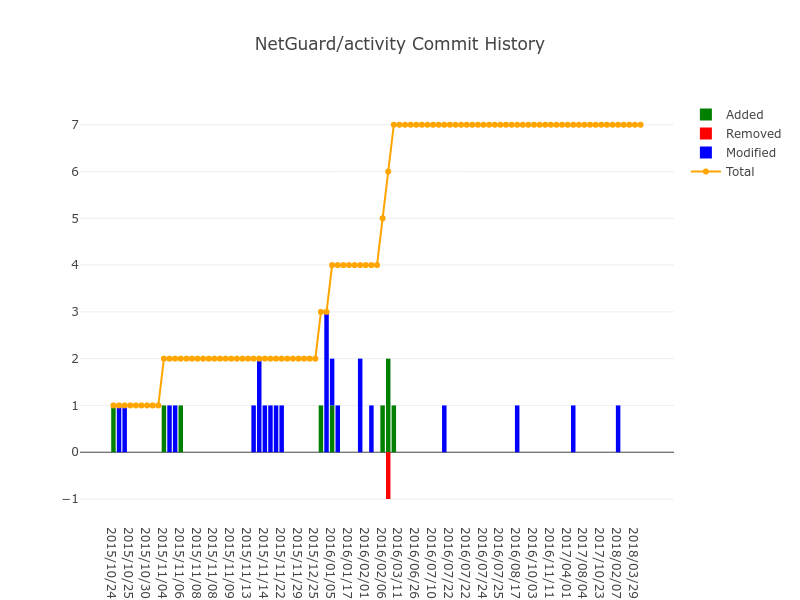
\includegraphics[width=\linewidth,height=0.5\linewidth]{imgs/NetGuard_activity_history.png}
\caption{Histórico das activities do repositório NetGuard}
\label{fig:repoactivity}
\end{figure}


Nas Figuras de \ref{fig:repobroadcast} a \ref{fig:repopermission} podemos ver os históricos dos outros componentes para o mesmo repositório.

%figura dos broadcasts.
\begin{figure}[H]
\centering
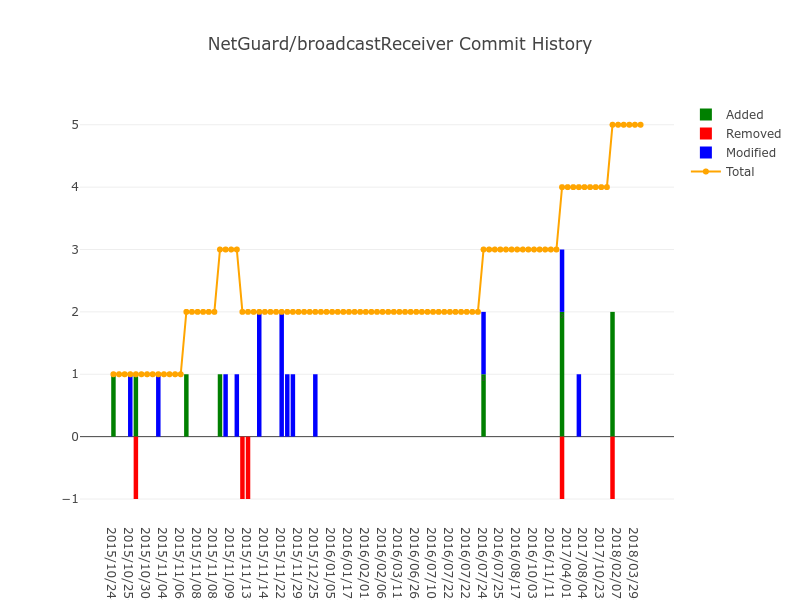
\includegraphics[width=\linewidth,height=0.5\linewidth]{imgs/NetGuard_broadcastReceiver_history.png}
\caption{Histórico dos broadcast receivers do repositório NetGuard}
\label{fig:repobroadcast}
\end{figure}

%figura dos providers.
\begin{figure}[H]
\centering
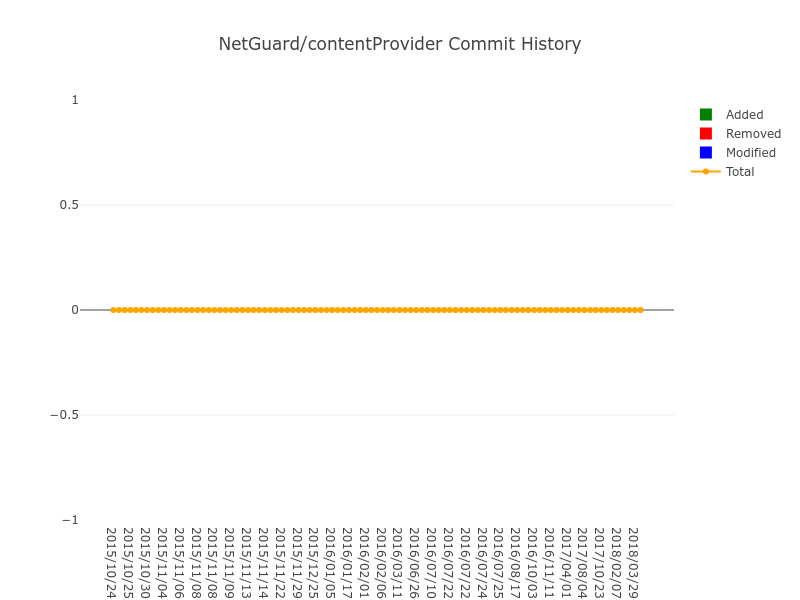
\includegraphics[width=\linewidth,height=0.5\linewidth]{imgs/NetGuard_contentProvider_history.png}
\caption{Histórico dos content providers do repositório NetGuard}
\label{fig:reporeceiver}
\end{figure}

%figura dos services.
\begin{figure}[H]
\centering
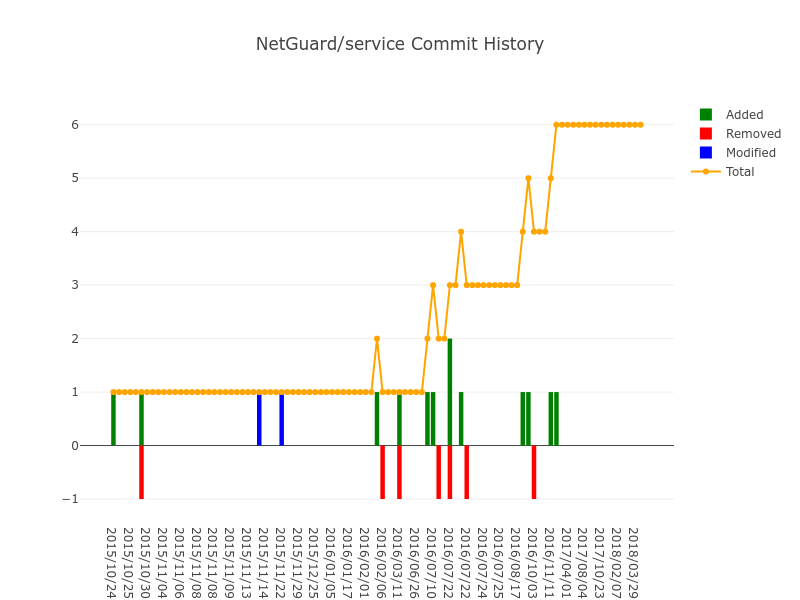
\includegraphics[width=\linewidth,height=0.5\linewidth]{imgs/NetGuard_service_history.png}
\caption{Histórico dos services do repositório NetGuard}
\label{fig:reposervice}
\end{figure}

%figura das uses perm.
\begin{figure}[H]
\centering
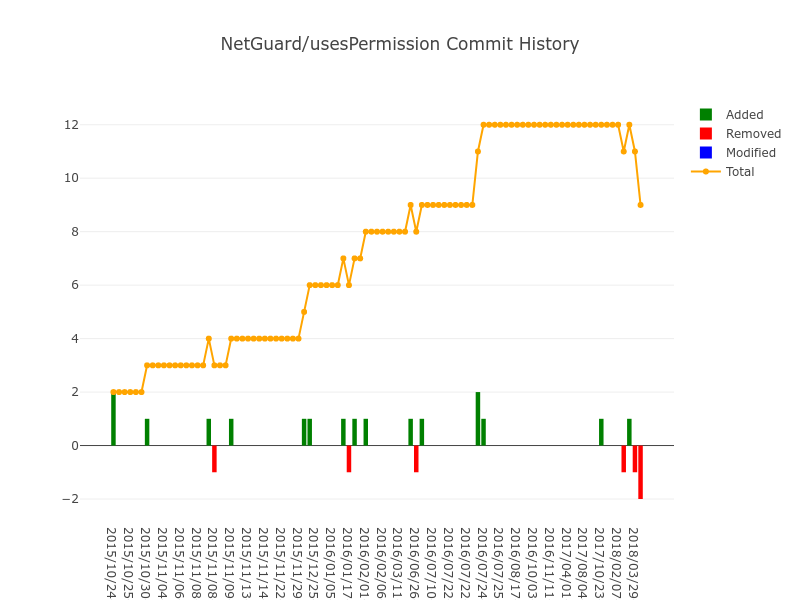
\includegraphics[width=\linewidth,height=0.5\linewidth]{imgs/NetGuard_usesPermission_history.png}
\caption{Histórico das permissões utilizadas no repositório NetGuard}
\label{fig:repouses}
\end{figure}

%figura das permissions.
\begin{figure}[H]
\centering
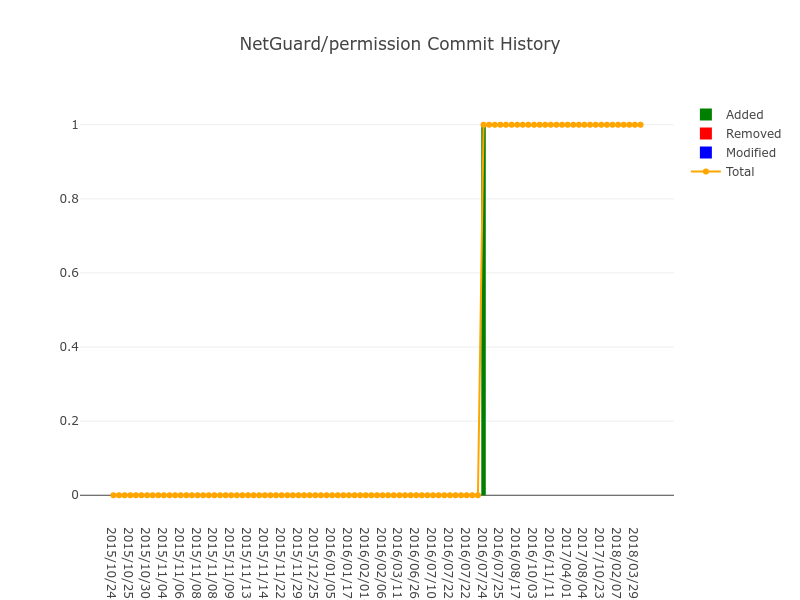
\includegraphics[width=\linewidth,height=0.5\linewidth]{imgs/NetGuard_permission_history.png}
\caption{Histórico das permissões criadas pelo repositório NetGuard}
\label{fig:repopermission}
\end{figure}




%=============================
%=         Conclusão         =
%=============================
\newpage

\section{Conclusão}%24-25
%\subsection{Trabalhos Futuros}
%Extender a ferramenta para analisar também o codigo fonte e valida-lo junto ao manifesto.

Após os experimentos realizados, podemos concluir que a implementação da ferramenta proposta no começo do semestre foi bem sucedida. Por mais que alguns repositórios, 57 para ser exato, tenham apresentado problemas durante a mineração, outros 1138 foram processados com sucesso, conforme foi comentado em \ref{sec:experimentos}.

Na seção a seguir, apresentamos alguns trabalhos que poderiam fazer uso de uma ferramenta deste tipo. E na seção seguinte, sugerimos alguns trabalhos futuros que visam evoluir a ferramenta proposta.


%================TRABALHOSRELACIONADOS===================
%\newpage
\subsection{Trabalhos Relacionados}%18-20

Em \cite{Calciati}, Calciati e Gorla realizaram um estudo sobre como as requisições de permissões evoluíram ao longo das várias releases das aplicações. Eles extraíram essa informação do arquivo APK, a versão final da aplicação que é baixada pelos dispositivos dos usuários. Este trabalho poderia ser enriquecido com informações a respeito do desenvolvimento do código fonte das aplicações com o uso da ferramenta proposta. \\

Isto pode ser visto em \cite{WhoAdded}, onde Krutz \textit{et al} desenvolveram uma ferramenta semelhante, denominada oSARA, para avaliar quem realizava as alterações nas permissões das aplicações. Em comparação com oSARA, a ferramenta proposta é capaz de coletar informações sobre outros componentes Android além das permissões.\\

\subsection{Trabalhos Futuros}

%Listar 2-3 melhorias ou novas funcionalidades que podem ser feitas na ferramenta.


%avaliar o codigo fonte validando junto ao manifesto
Hoje a ferramenta extrai dados da aplicação olhando apenas para o seu arquivo de manifesto. Em um trabalho futuro ela pode ser estendida para analisar também o código fonte e validá-lo junto ao manifesto. Dessa forma, além de sabermos em que momento um componente foi acrescentado no arquivo XML, também saberíamos em que momento a classe que o representa foi implementada.

%avaliar codigo fonte em funcao do framework android

Uma outra opção de melhoria da ferramenta seria utilizá-la para obter dados sobre a implementação de outros elementos Android, como por exemplo, {\small\textbf{\texttt{AlarmManagers}}}, {\small\textbf{\texttt{AsyncTasks}}} e {\small\textbf{\texttt{Notifications}}}. Que apesar de não serem declarados no manifesto, são muito utilizados pelas aplicações para agendar procedimentos, executar tarefas assíncronas e exibir notificações para o usuário, respectivamente.

%portar para python 

Na Seção \ref{sec:resultados} apresentamos um resumo dos dados obtidos pela ferramenta que foi gerado por um script Python. Uma abordagem diferente seria utilizar os arquivos CSV para gerar um banco de dados baseado em grafos e a partir disso realizar querys relativas aos dados desejados. 


%================Bibliografia===================
%referencias
\newpage
%\bibliographystyle{IEEEtranS}
\bibliographystyle{ieeetr}
\bibliography{lib}
\nocite{developer}

\end{document}
